\section{External Architecture}
Two external architectures will be covered: The launcher architecture, and the \guicomponents[] library architecture.

\subsection{Launcher}
The external architecture for the launcher, can be seen in \autoref{fig:external_architecture}.
\begin{figure}[h]
	\centering
	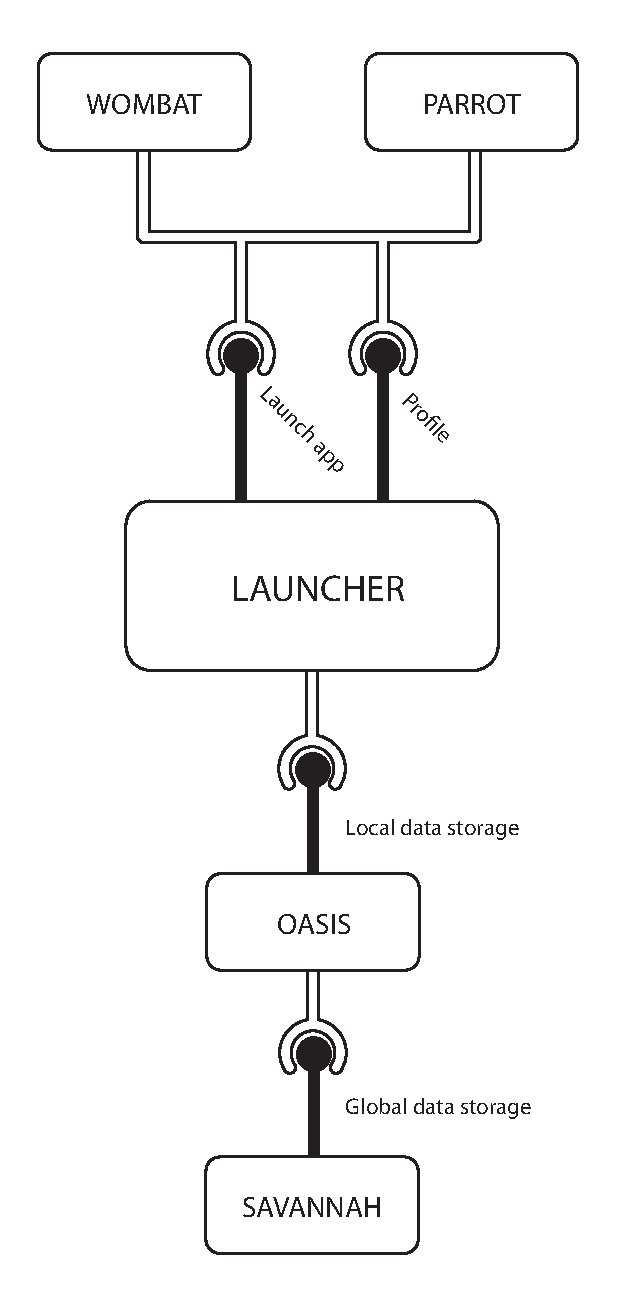
\includegraphics[width=0.5\textwidth]{gfx/external_architecture.pdf}
	\caption{External Architecture}
	\label{fig:external_architecture}
\end{figure}
The launcher provides with two services: Launching apps, and providing information about the profile that is authenticated. The \textit{Launch app} service allows external apps to run and be stopped, ie: \textit{launch}.
The \textit{Profile} service provides the possibility of external apps to retrieve the current authenticated profile.
This is necessary for external apps in order to use the profile specific data in Oasis.

The Oasis database is the single required service provider for the launcher.
It allows for authenticating profiles and store settings for the launcher relative to the profile.

\subsection{\guicomponents[]}
The \guicomponents[] architecture is not final, and is based on existing Android architecture. An example of the architecture can be seen in \autoref{fig:gui_comp_architecture}. The philosophy behind the architecture is to use existing Android UI components, with a new layout and possible added functionality. The example shown in \autoref{fig:gui_comp_architecture} highlights a possible way incooperate this philosophy, assuming the need for a customized button \textit{GButton}. 
\begin{figure}[h]
	\centering
	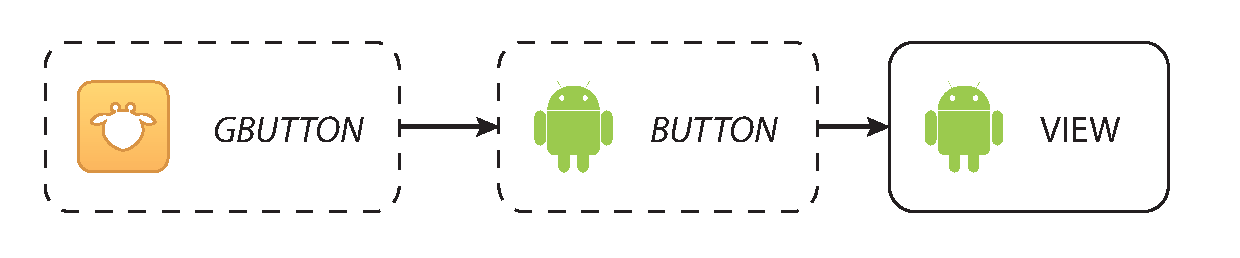
\includegraphics[width=1\textwidth]{gfx/gui_components_architecture.pdf}
	\caption{\guicomponents[] Architecture Example}
	\label{fig:gui_comp_architecture}
\end{figure}

